\documentclass{article} % Defines the document class, article is commonly used
\usepackage[shortlabels]{enumitem}
\usepackage{amsmath}    % Allows for more advanced math formatting
\usepackage{amssymb}    % Provides additional mathematical symbols
\usepackage{amsthm}     % \qed
\usepackage{graphicx}   % image
\usepackage{float}      % image placement
\usepackage{hyperref}
\hypersetup{
    colorlinks=true,       % false: boxed links; true: colored links
    linkcolor=black,       % color of internal links
}
\usepackage[margin=0.5in]{geometry}

\begin{document}

\title{EEC133 Midterm Formula Sheet}
\author{Tao Wang}
\date{\today}

\maketitle

\begin{figure}[H]
    \centering
    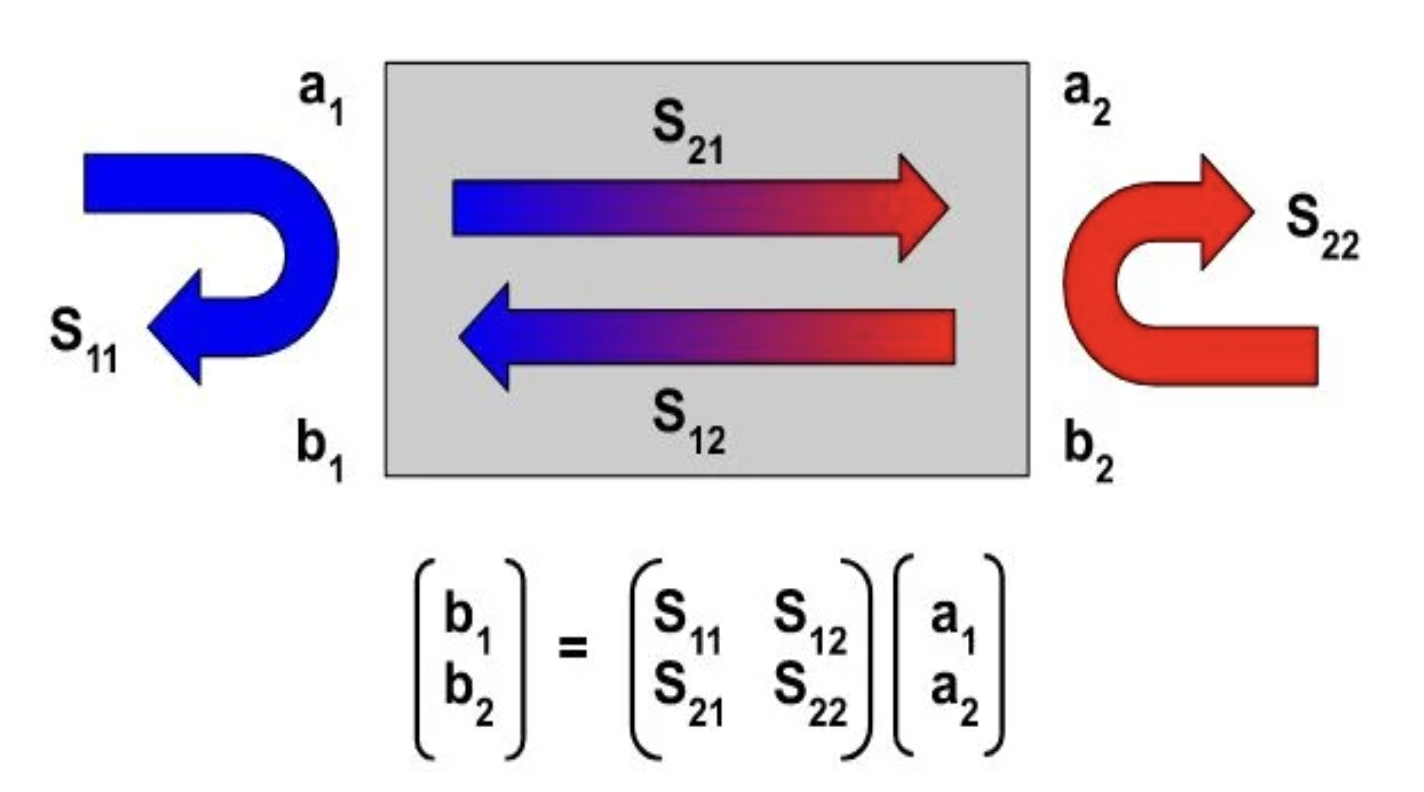
\includegraphics[width=0.4\textwidth]{./image/figure1.png}
    \caption{S Parameter}
\end{figure}

\textbf{db to dbm}
\[P(\text{dBm}) = 10 \times \log(P(w)) + 30\]

\textbf{Steradian:}
\[A = r^2 \Omega\]

\begin{center}
    where A is the surface area patch, $r$ is the radius, and $\Omega$ is the solid angle.
\end{center}

\textbf{Total Radiation Power (W)}
\begin{quote}
    \[P_{rad} = \int U(\theta, \phi) d\Omega\]
\end{quote}

\textbf{Half Power Beamwidth:}
\[\theta_2 - \theta_1\]

\begin{center}
    where $\theta_2, \theta_1$ are the angles where the normalized radiation intensity is $\frac{1}{2}$.
\end{center}
\[\Omega_A \approx \frac{4\pi}{D_0}\]

\textbf{Directivity (1/steradian):}

\[D_0 = \frac{4 \pi}{\Omega_p} = \frac{4 \pi}{\int_{sphere} F(\theta, \phi) d\Omega}\]

\begin{center}
    where $\Omega_p$ is the pattern solid angle.
\end{center}

\[\frac{A_e}{D_0} = \frac{\lambda^2}{4 \pi}\]

\begin{center}
    where $A_e$ is the effective area of the antenna, $D_0$ is the directivity of the antenna, and $\lambda$ is the wavelength of the wave transmitted by the antenna.
\end{center}

\textbf{Gain}
\[G_0 = e \times D_0\]

\begin{center}
    where $e$ is the efficiency of the antenna.
\end{center}

\textbf{Angular Resolution}
\begin{quote}
    \[\frac{\lambda}{\text{Aperture Size}} = \frac{\lambda}{d}, \text{ where d is the diameter of the dish}\]

\end{quote}

\textbf{Poynting Vector}
\[\vec{S}_{av} = \hat{z}\frac{|\widetilde{E}|^2}{2 \eta}\]

\textbf{Power Radiated from the Antenna}
\[|\vec{S}_{avg}| = \frac{e_t P_{t}}{4 \pi r^2}D_t\]

\textbf{Friss Transmission Equation:}
\[\frac{P_{rec}}{P_t} = e_t e_r \left(\frac{\lambda}{4\pi R}\right)^2 D_t D_r\]
\[=\left(\frac{\lambda}{4\pi R}\right)^2 G_t G_r\]
\[=\frac{e_r e_t A_t A_r}{\lambda^2 R^2}\]

\begin{center}
    where subscript t denotes the transmitter's parameter, r denotes the receiver's parameter, and R is the distance between two antennas.
\end{center}

\textbf{Vector Potential}
\[\vec{H} = \frac{1}{\mu_0} \nabla \times \vec{A}\]

\[\vec{E} = -\nabla \phi - \frac{\partial \vec{A}}{\partial t}\]

\textbf{Gauge}

\[\phi_{new} = \phi - \frac{\partial \psi}{\partial t}\]

\[\vec{A}_{new} = \vec{A} + \nabla \psi\]

\[\text{Coulomb Gauge: } \nabla \cdot \vec{A} = 0\]

\[\text{Lorenz Gauge: } \nabla \cdot \vec{A} = \frac{-1}{c^2} \frac{\partial \phi}{\partial t}\]


\textbf{Retarded Potential}
\[\widetilde{A}(\vec{r}) = \int \frac{\mu_0 \widetilde{J}(\vec{r})e^{-jkr}}{4\pi R} dV'\]



\textbf{Hertzian Dipole Antenna:}
$l < \frac{\lambda}{50}$

Far Field ($r >> \lambda$)

\[\widetilde{E}_{ff, \theta} = j \eta_0 \frac{I k l}{4 \pi r} e^{-jkr} \sin(\theta)\]
\[\widetilde{H}_{ff, \phi} = \frac{\widetilde{E}_{ff, \theta}}{\eta_0}\]
\[D(\theta, \phi) = 1.5 \sin^2(\theta)\]
\[F(\theta, \phi) = \sin^2(\theta)\]
\[P_{rad} = 40 \pi^2 I_0^2\left(\frac{l}{\lambda}\right)^2\]
\[R_{rad} = 80 \pi^2 \left(\frac{l}{\lambda}\right)^2\]

\textbf{Small dipole Antenna}: $l < \frac{\lambda}{10}$

Fields are 1/2 those form the Hertzian Dipole.

\[P_{rad} = 10 \pi^2 I_0^2\left(\frac{l}{\lambda}\right)^2\]
\[R_{rad} = 20 \pi^2 \left(\frac{l}{\lambda}\right)^2\]

\[\text{Resonance Dipole Length: } L = \frac{\lambda}{2} + n\lambda, n \geq 0\]

\textbf{Small Loop Antenna:}
$a << \frac{\lambda}{6 \pi}$

Far Fields ($r >> \lambda$)

\[\widetilde{H}_{ff, \theta} = \frac{I k^2 (\pi a^2) }{4 \pi r} e^{-jkr}\sin(\theta)\]
\[\widetilde{E}_{ff, \phi} = -\widetilde{H}_{\theta} \eta_0\]

\[D(\theta, \phi) = 1.5 \sin^2(\theta)\]
\[R_{rad} = 320 \pi^6 \left(\frac{a}{\lambda}\right)^4 N^2\]

Choosing Capacitor to be in parallel with loop antenna to cancel antenna's input reactance
\[j\omega C - j \frac{X_A}{R_A^2 + X_A^2} = 0\]

\begin{center}
    where $X_A$ is the input reactance and $R_A$ is the input resistance of the antenna
\end{center}

\textbf{Two Hertzian Dipole Antenna}
\begin{quote}
    \[\widetilde{E}_{ff}(\vec{r}) \bigg|_{\theta = \pi / 2} = \hat{\theta} \frac{j \eta_0 k l d}{4 \pi r}e^{-jkr} \left(e^{jk\frac{l}{2}\cos(\phi)} + A e^{j \alpha} e^{-jk \frac{l}{2} \cos(\phi)}\right), \text{where l is the distance between two Hertzian Dipoles and A is the ratio between currents in the dipoles}\]

    \[\widetilde{H}_{ff}(\vec{r}) \bigg|_{\theta = \pi / 2} = \hat{\phi} \frac{j k l d}{4 \pi r}e^{-jkr} \left(e^{jk\frac{l}{2}\cos(\phi)} + A e^{j \alpha} e^{-jk \frac{l}{2} \cos(\phi)}\right)\]

    \[\vec{S}(\vec{r}) \bigg|_{\theta = \pi/2} = \hat{r} \eta_0 \left|\frac{kld}{4\pi r}\right|^2 \left|e^{jk\frac{l}{2}\cos(\phi)}+Ae^{j\alpha}e^{-jk \frac{l}{2}\cos(\phi)}\right|^2\]

    \[D(\theta, \phi) = \frac{3}{2}\left(\frac{1 + A^2 + 2A \cos[kl\cos(\phi) - \alpha]}{f(A, \phi)}\right)\]

    \[F(\theta, \phi) = \left(\frac{1 + A^2 + 2A \cos[kl\cos(\phi) - \alpha]}{(1 + A)^2}\right)\]
\end{quote}

\textbf{Patch Antenna}
\begin{quote}
    \[f = \frac{c}{2\sqrt{\epsilon_r}L}\]
    \[W = 1.5 L\]
\end{quote}

\textbf{Aperture Antenna}
\begin{quote}
    \[\beta_{xz} = 2 \theta = 0.38 \frac{\lambda}{l_x}\]
    \[\beta_{yz} = 2 \theta = 0.88 \frac{\lambda}{l_y}\]
    \[D_0 = \frac{4 \pi}{\text{Beam Solid Angle}}\]
\end{quote}

\textbf{Other}
\begin{quote}
    \[\text{Reflection Coefficient}: \gamma = \frac{Z_L - Z_0}{Z_L + Z_0}\]
    \[\text{Transmission Line Input Impedance}: Z_{in} = Z_0\left(\frac{Z_L + jZ_0 \tan(kl)}{Z_0 + jZ_L\tan(kl)}\right)\]
    \[\text{Power Flowing Through a Transmission Line}: P_{avg} = \frac{|V_0 ^+|^2}{Z_0} (1 - |\gamma|^2)\]
    \[\text{Standing Wave Ratio}: S = \frac{1 + |\gamma|}{1 - |\gamma|}\]
\end{quote}

\end{document}
